\documentclass[11pt]{cernrep} \usepackage{graphicx,epsfig} \bibliographystyle{lesHouches}

\begin{document}

\section{Ratio of the Z to gamma transverse momentum differential cross-section \protect\footnote{Section
    coordinator:V.~Ciulli} $^{,}$ ~\protect\footnote{Contributing authors: M.~Chiesa, J.~Lindert, A.~Marini,  
    G.~Montagna, M.~Moretti, O.~Nicrosini, F.~Piccinini, E.~Takasugi, M.~A.~Weber }}

The ratio of the associated production of a $\mathrm{Z}/\gamma^*$ or a $\gamma$ with one or more jets has been recently measured in
proton-proton collisions at 8 TeV center-of-mass energy by the CMS Collaboration at the CERN
LHC~\cite{Khachatryan:2015ira}. In the limit of high transverse momentum of the vector boson $p_T^{V}$
($V=Z,\gamma$) and at leading order (LO) in perturbative quantum chromodynamics (QCD), effects due to the mass of the Z
boson ($m_\mathrm{Z}$) are small, and the 
cross section ratio of Z+jets to $\gamma$+jets as a function of $p_T^{V}$ is expected to become constant, reaching a
plateau for $p_T^{V} \geq 300$ GeV~\cite{StirlingPaperZGamma}. (Hereafter, production of $Z/\gamma^*$ + jets is denoted by
Z+jets.) A QCD calculation at next-to-leading order (NLO) for pp$\to$Z+jets and pp$\to\gamma$+jets was provided by
the {\tt BLACKHAT} Collaboration~\cite{BlackHat}.  The NLO QCD corrections tend to decrease the value of
the cross section ratio. At higher energies, electroweak (EW) corrections 
can also introduce a dependence of the cross section on logarithmic terms of the form
$\ln(p_T^{\mathrm{Z}}/m_{\mathrm{Z}})$ that become large and pose a challenge for perturbative calculations.  

Searches for new particles involving final states characterized by the presence of large missing transverse
energy and hard jets, use the $\gamma$+jets process to model the invisible Z decays, Z$\to\nu\bar{\nu}$, since the
$\gamma$+jets cross section is larger than the Z+jets process where the Z decays to leptons. A precise estimate of EW
corrections on the cross section ratio for Z+jets and $\gamma$+jets is therefore crucial to reduce uncertainties related
to the Z$\to\nu\bar{\nu}$ background estimation in these searches. 

In the CMS measurement~\cite{Khachatryan:2015ira}, results are unfolded into a fiducial region defined at particle
level. For Z+jets events, the leading leptons are required to have $p_T>20$ GeV and $|\eta|<2.4$, 
while jets are required to have $p_T>30$ GeV within the region of $|\eta|<2.4$. Electrons and muons have different
energy losses due to final state radiation at particle level. In order to compensate for these differences, a
``dressed'' level is defined to make the electron and muon channels compatible to within 1\%. This is achieved by
defining in simulation a particle momentum vector by adding the momentum of the stable lepton and the momenta of all
photons with a radius of $\Delta R=0.1$ around the stable lepton. All jets are required to be separated from each lepton
by $\Delta R>0.5$. At the particle level, a true isolated photon is defined as a prompt photon, around which the scalar
sum of the $p_T$ of all stable particles in a cone of radius $\Delta R=0.4$ is less than 5 GeV. A true isolated photon
is defined as a prompt photon (not generated by a hadron decay), around which the scalar sum 
of the $p_T$ of all stable particles in a cone of radius $\Delta R=0.4$ is less than 5 GeV. When comparing the
cross sections for Z+jets and $\gamma$+jets, the rapidity range of the bosons
is restricted to $|{y^{V}}|<1.4$ because this is the selected kinematic region for the photons.
The ratio of the differential cross sections as a function of $p_T$ is measured
in the phase space regions: $N_{\mathrm{jets}}\geq 1,\,2,\,3$, and $H_T>300$ GeV, $N_{\mathrm{jets}}\geq1$. 

\begin{figure}
\begin{center}
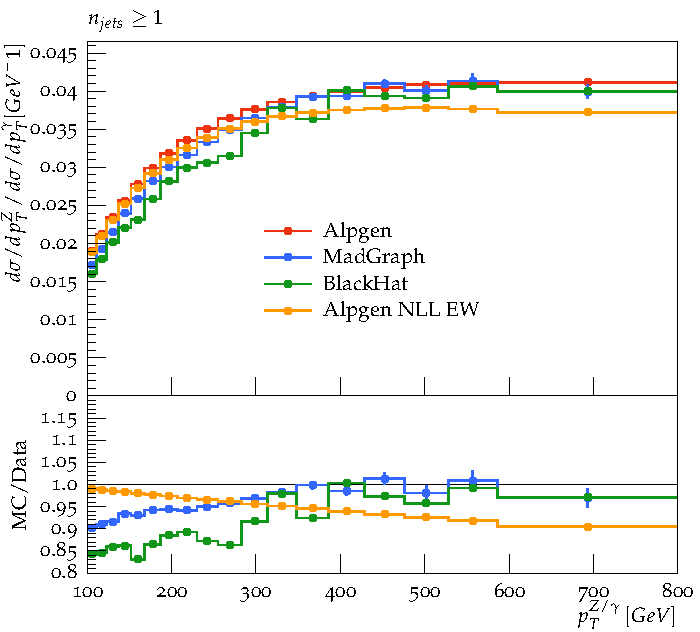
\includegraphics[width=0.5\textwidth]{d07-x01-y01-mc.pdf} \\
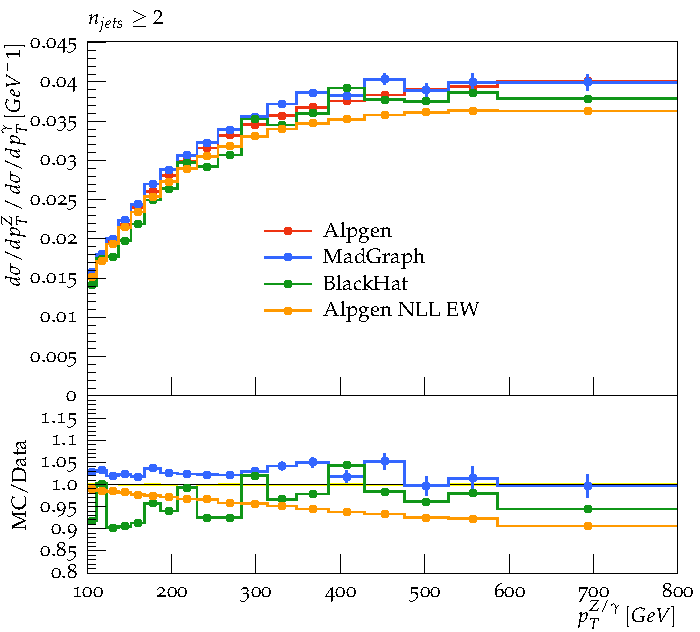
\includegraphics[width=0.5\textwidth]{d08-x01-y01-mc.pdf} \\
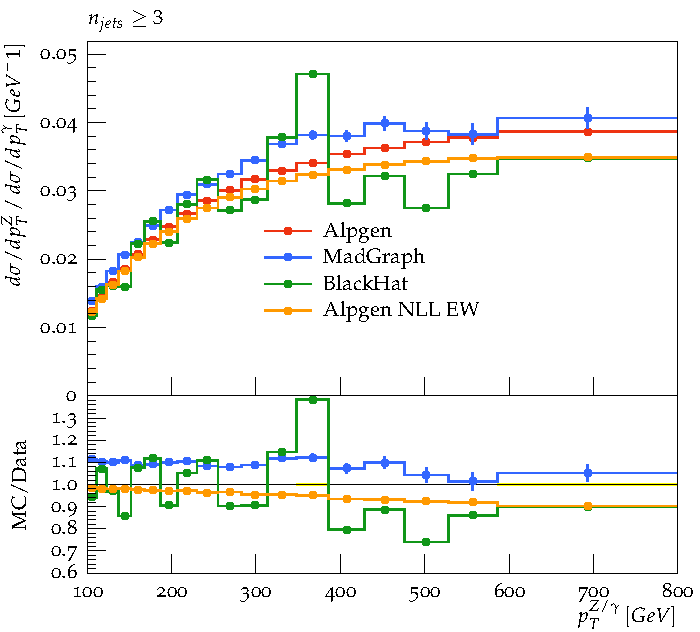
\includegraphics[width=0.5\textwidth]{d08-x02-y01-mc.pdf}
 \caption{Comparison of different predictions for the ratio of Z+jets over $\gamma$ + jets at 8 TeV pp
   center-of-mass energy. From top to bottom, results are shown for events with at least 1, 2 and 3 jets accompaning the
   boson. For fixed order predictions this value corresponds to the number of partons in the final state at the lowest order.}
\label{zgrmc}
\end{center}
\end{figure}

Figure~(\ref{zgrmc}) compares several predictions for the ratio within the fiducial regions as defined above~\footnote{We dropped
the comparison for $H_T>300$ GeV because fixed order predictions are known to fail describing high jet activity with a
comparatively low vector boson $p_T$.}. The fixed
order partonic predictions computed with the {\tt ALPGEN} generator are shown at LO and at 
approximated NLO accuracy~\cite{Chiesa:2013yma}, \emph{i.e.} including the effect of virtual weak corrections in the Sudakov approximation obtained by
means of the algorithm of Refs.~\cite{Denner:2000jv,Denner:2001gw}, as described in the previous paragraphs. The
predictions for $Z+$~jets and $\gamma+$~jets are computed in the $G_{\mu}$ and $\alpha_0$ schemes, respectively, with
the set of parameters listed above for the calculation of the $\mathcal{O}(\alpha)$ corrections to the process
$W+2$~jets. The factorization scale is set to $\sum_j p_T^j +\sqrt{M^2(V) +p^2_T(V)}$. CTEQ5L is used as
PDF set: it is worth noticing, however, that PDFs largely cancel in the $Z/\gamma$ ratio as pointed out in
Ref.~\cite{Ask:2011xf}.  More precisely, the predictions for $\gamma+$~jets and $Z+$~jets are computed by using the {\tt
phjet} and {\tt zjet} packages, respectively: at variance with the {\tt vbjet} package, where the external vector bosons
are produced on-shell, in {\tt zjet} the $Z$ boson decays in a fermion-antifermion pair including all the off-shell and
spin correlation effects. These packages include only the QCD contributions of order $\alpha_S^{n \, {\rm jets}} \alpha$
to the LO predictions. Though the LO results for $Z+$~jets include exactly off-shell and spin correlation effects, the
Sudakov corrections are obtained in the on-shell approximation by using the phase space mapping described in
Ref.~\cite{Denner:2014ina}.

The other predictions are also shown in the CMS paper, where a detailed description of the configuration used can be
found. For Z+jets and $\gamma$+jets generated with the {\tt MADGRAPH5}~\cite{MadGraph5} program, the leading-order
multiparton matrix element calculation includes up to four partons in the final state. The
showering and hadronization, as well as the underlying event, are modeled by {\tt PYTHIA6}~\cite{pythia6}. The events
are generated with the CTEQ6L1~\cite{CTEQ6} parton distribution functions and the ktMLM
matching scheme~\cite{MatchingPaper} with a matching parameter of 20 GeV is applied.  
In addition to these Monte Carlo signal data sets, a NLO perturbative QCD calculation from the
{\tt BLACKHAT} Collaboration~\cite{BlackHat} is available for a boson accompanied by up to three jets. These
calculations use MSTW2008nlo68cl~\cite{MSTW} with $\alpha_{S}=0.119$ as the PDF set, and the renormalization and
factorization scales are set to $\mu_{R}=\mu_{F}=H_T+E_T^{\mathrm{V}}$, where $H_T$ is the scalar $p_T$ sum of all
outgoing partons with $p_T>20$ GeV and $E_T^{\mathrm{V}}$ is defined as
$\sqrt{m_{\mathrm{Z}}^{2}+\left(p_T^{\mathrm{Z}}\right)^{2}}$ and $p_T^{\gamma}$, respectively, for Z+jets and $\gamma$+jets.
In addition, the photons must satisfy the Frixione cone isolation condition~\cite{Frixione}.

From the plot it is clear that both NLO QCD and EWK corrections are negative with respect to the fixed order LO
predictions. The NLO QCD corrections are larger for lower transverse momentum of the bosons, reaching a 15\% effect for
$N_{\mathrm{jets}} \geq 1$. A fraction of this effect seems to be included by {\tt MADGRAPH} predictions, which include higher order
real parton emissions in the matrix-element calculation. The EWK corrections increase with the boson transverse
momentum, up to about 10\% for $p_T > 600$ GeV in events with at least one jet. Both QCD and EWK corrections decrease
for larger jet multiplicities. It can be also noticed that {\tt MADGRAPH} prediction overshoot the NLO QCD ones for
larger multiplicities. 

\begin{figure}
\begin{center}
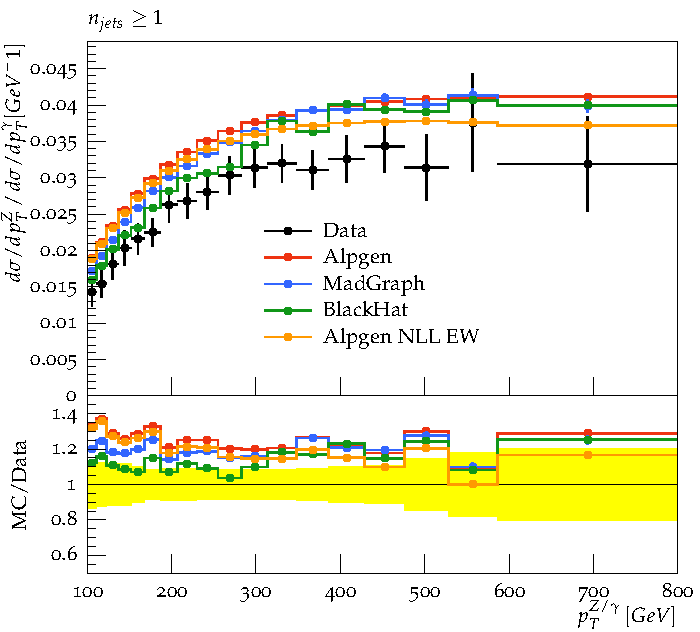
\includegraphics[width=0.5\textwidth]{d07-x01-y01.pdf} \\
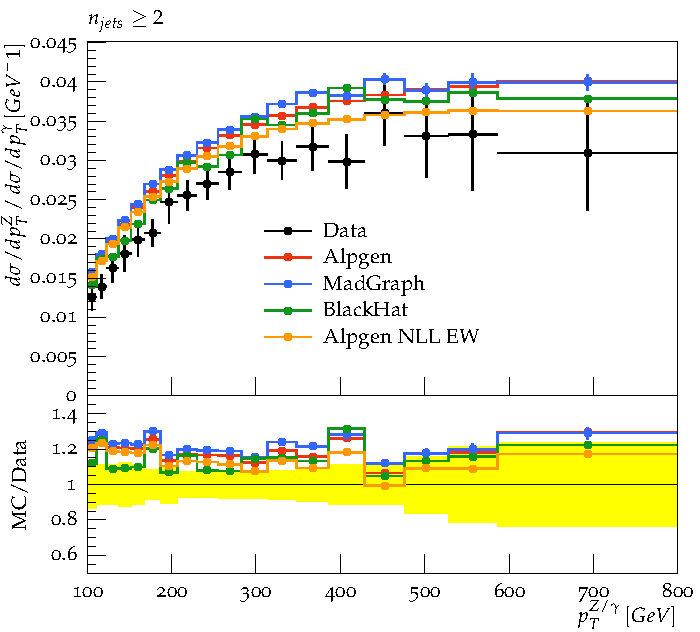
\includegraphics[width=0.5\textwidth]{d08-x01-y01.pdf} \\
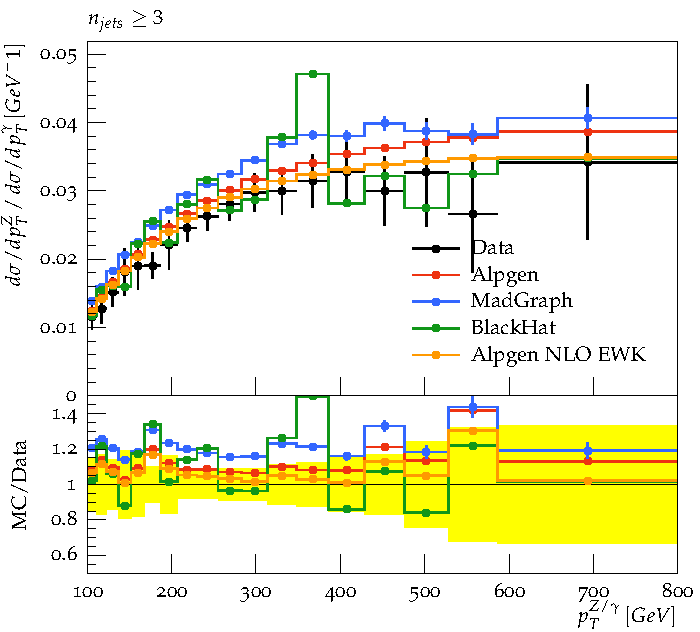
\includegraphics[width=0.5\textwidth]{d08-x02-y01.pdf}
 \caption{Comparison to CMS data of different predictions for the ratio of Z+jets over $\gamma$ + jets at 8 TeV pp
   center-of-mass energy. From top to bottom, results are shown for events with at least 1, 2 and 3 jets accompaning the
   boson. For fixed order predictions this value corresponds to the number of partons in the final state at the lowest order.}
\label{zgrdata}
\end{center}
\end{figure}

In Figure~(\ref{zgrdata}), these predictions are compared to CMS results, showing that the agreement improves
when NLO corrections are included, both in the case of QCD and EWK ones. In particular, including the EWK corrections,
results are in better agreement in the high boson transverse momentum region, especially for larger jet multiplicities. 

\begin{figure}
\begin{center}
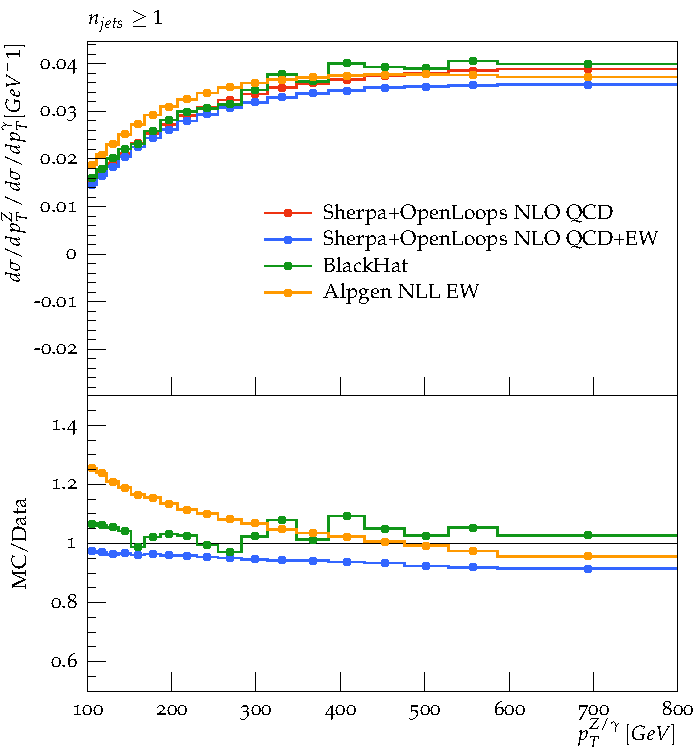
\includegraphics[width=0.5\textwidth]{d07-x01-y01-SherpaOL-mc.pdf} \\
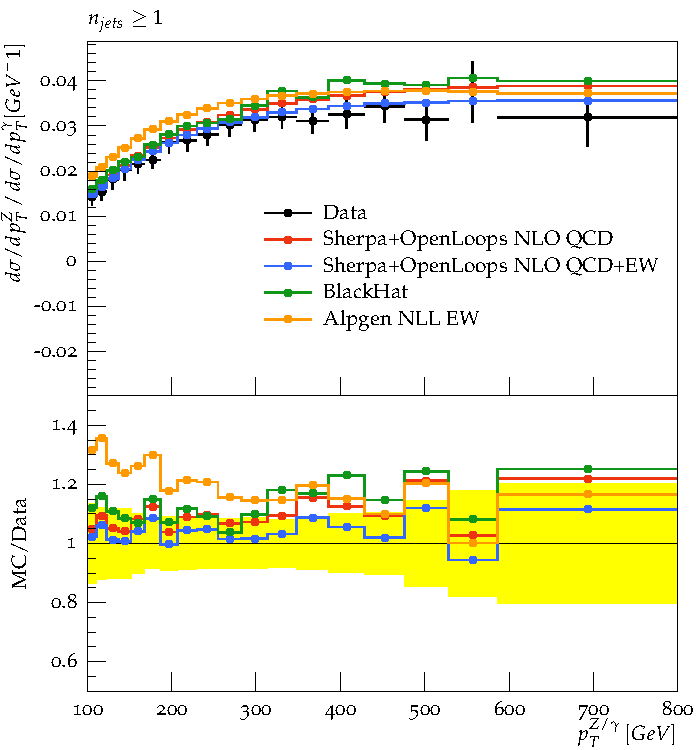
\includegraphics[width=0.5\textwidth]{d07-x01-y01-SherpaOL.pdf} \\
 \caption{Comparison of different predictions at NLO QCD,  NLL EW and NLO QCD+EW order for the 
   ratio of Z + jets over $\gamma$ + jets at 8 TeV pp
   center-of-mass energy, in events with at least 1 jet accompaning the
   boson. For fixed order predictions this value corresponds to the
   number of partons in the final state at the lowest order. Top plot
   shows a comparison among the predictions. The bottom plot shows a comparison to CMS data. } 
\label{zgrNLO}
\end{center}
\end{figure}

In addition Figure~\ref{zgrNLO} shows, for events with a vector boson and at least one
jet, fixed-order predictions from {\tt Sherpa+OpenLoops}. The $Z$+jets prediction
is obtained from an off-shell calculation for $\ell^+\ell^-$+jets including all $Z/\gamma^*$ interference effects.
The presented predictions are based on the recently 
achieved automation of NLO QCD+EW 
calculations~\cite{Kallweit:2014xda,Kallweit:2015dum}, as described in 
Section~\ref{put_label_of_section}. Related predictions for the $Z$+jets/$\gamma$+jets 
ratio (with an on-shell $Z$ boson) from {\tt Munich+OpenLoops} have already been presented 
in~\cite{Kallweit:2015fta} and have for example been employed for background 
predictions in \cite{CMS:2015jdt}. Here, we employ NNPDF2.3QED \cite{Ball:2013hta} 
parton distributions with $\alpha_S=0.118$ and all input parameters and scale 
choices are as detailed in~\cite{Kallweit:2015dum}. In particular, all unstable 
particles are treated in the complex-mass scheme~\cite{Denner:2005fg} and  
renormalisation and factorisation scales are set to 
$\mu_{R,F}=\hat{H}_{\mathrm{T}}'/2$, where $\hat{H}_{\mathrm{T}}'$ is the scalar 
sum of the transverse energy of all parton-level final-state objects, 
$\hat{H}_{\mathrm{T}}' = \sum_{i\in \{\mathrm{quarks,gluons}\}} p_{\mathrm{T},i} 
+ p_{\mathrm{T},\gamma} + E_{\mathrm{T}, V}$. QCD partons and photons that are 
radiated at NLO are included in $\hat{H}_{\mathrm{T}}'$, and the vector-boson 
transverse energy, $E_{\mathrm{T},V}$,  is computed using the total (off-shell) 
four-momentum of the corresponding (dressed) decay products, i.e. 
$E^2_{\mathrm{T},Z}=p^2_{\mathrm{T},\ell\ell}+m_{\ell\ell}^2$ and 
$E^2_{\mathrm{T},\gamma}=p_{\mathrm{T},\gamma}^2$. The weak coupling constant 
$\alpha$ is renormalized in the $G_{\mu}$ scheme for the $\ell^+\ell^-$+jets prediction, 
while the $\alpha(0)$-scheme is used for the $\gamma$+jets prediction. Results 
are presented at the NLO QCD level and combining QCD and EW corrections via an 
additive prescription, i.e. $\sigma^{\mathrm{NLO}}_{\mathrm{QCD+EW}} =
\sigma^{\mathrm{LO}}+\delta\sigma^{\mathrm{NLO}}_{\mathrm{QCD}} + 
\delta\sigma^{\mathrm{NLO}}_{\mathrm{EW}}$. Isolated photons in the $\gamma$+jets 
predictions are required to satisfy Frixione cone isolation~\cite{Frixione} with parameters
as specified in \cite{Khachatryan:2015ira}.

The agreement of the combined NLO QCD+EW prediction with the CMS data is
remarkable over the whole spectrum. As already noted, at low transverse momentum
NLO QCD corrections to the ratio are relevant due to mass effects, but sizable
EW corrections due to EW Sudakov logarithms (of different size for the two
processes) alter the shape of the ratio prediction already much below 1 TeV.
These results show the importance of combining NLO QCD and EW corrections in a
unified framework.


\bibliography{zgammaratio}

\end{document}
